
\de{ĐỀ THI GIỮA HỌC KỲ II NĂM HỌC 2022-2023}{THPT Trường Chinh - Đề A}

\begin{bt}%[0T7B2-1]%[Dự án đề kiểm tra HKII NH22-23- BCTuan]%[THPT Trường Chinh đề A]
Lập bảng xét dấu và giải bất phương trình: $5x^2+2x-7>0$.
\loigiai{
	Bảng xét dấu của biểu thức $f(x)=5x^2+2x-7$ như sau
	\begin{center}
		\begin{tikzpicture}
			\tkzTabInit[lgt=1.2,espcl = 3,deltacl=0.6]
			{$x$ /0.8, $f(x)$ /0.8}
			{$-\infty$,$-\frac{7}{5}$,$1$,$+\infty$}
			\tkzTabLine{ ,+,0,-,0, +, }
		\end{tikzpicture}
	\end{center}
	Dựa vào bảng xét dấu ta có $5x^2+2x-7>0\Leftrightarrow \hoac{& x<-\dfrac{7}{5} \\ & x>1.}$\\
	Vậy tập nghiệm của bất phương trình là $S=\left(-\infty;-\dfrac{7}{5}\right)\cup (1;+\infty)$.
}
\end{bt}
\begin{bt}%[0T7B2-1]%[Dự án đề kiểm tra HKII NH22-23- BCTuan]%[THPT Trường Chinh đề A]
Tìm tất cả các giá trị của tham số $m$ để
	$2x^2-2(3m+1)x+3m+5>0$ nghiệm đúng với mọi số thực $x$.
	\loigiai{
Để $2x^2-2(3m+1)x+3m+5>0$ nghiệm đúng với mọi số thực $x$ khi và chỉ khi
$$\heva{& a>0 \\ & \Delta'<0}\Leftrightarrow \heva{& 2>0 \\ & (3m+1)^2-2(3m+5)<0}\Leftrightarrow 9m^2-9<0	\Leftrightarrow -1<m<1.$$
Vậy với $m\in (-1;1)$ thì $2x^2-2(3m+1)x+3m+5>0$ nghiệm đúng với mọi số thực $x$.
}
\end{bt}
\begin{bt}%[0T7B3-2]%[Dự án đề kiểm tra HKII NH22-23- BCTuan]%[THPT Trường Chinh đề A]
	Giải phương trình: $\sqrt{3x^2+x}=\sqrt{x^2+2x+6}$.
	\loigiai{
Ta có
\begin{eqnarray*}
	&&\sqrt{3x^2+x}=\sqrt{x^2+2x+6}\\
	&\Rightarrow &3x^2+x=x^2+2x+6\\
	&\Leftrightarrow & 2x^2-x-6=0\\
	&\Leftrightarrow &\hoac{& x=2 \\ & x=-\dfrac{3}{2}.}
\end{eqnarray*}	
Thay các nghiệm vừa tìm được vào phương trình ban đầu ta thấy đều thỏa mãn.\\
Vậy tập nghiệm của phương trình là $S=\left\{-\dfrac{3}{2};2\right\}$.
}
\end{bt}
\begin{bt}%[0T7K2-2]%[Dự án đề kiểm tra HKII NH22-23- BCTuan]%[THPT Trường Chinh đề A]
Một khung dây thép hình chữ nhật có chiều dài $20$ cm và chiều rộng $16$ cm được uốn lại thành khung hình chữ nhật mới có kích thước $(20-x)$ cm và $(16+x)$ cm. Với $x$ nằm trong các khoảng nào thì diện tích của khung sau khi uốn: tăng lên, không thay đổi, giảm đi?
\loigiai{
Ta có diện tích của khung ban đầu là $20\times 16=320$ (cm$^2$).\\
Điều kiện của biến $x$ là $0\le x<20$.\\
Diện tích khung sau khi uốn lại là $(20-x)(16+x)$.
\begin{itemize}
	\item Để diện tích khung tăng lên thì 
	$$(20-x)(16+x)>320\Leftrightarrow x^2-4x<0\Leftrightarrow 0<x<4.$$
	\item Để diện tích khung giảm đi thì
	$$(20-x)(16+x)<320\Leftrightarrow x^2-4x>0\Leftrightarrow \hoac{& x<0 \\ & x>4}\Leftrightarrow 4<x<20.$$
	\item Để diện tích khung không thay đổi thì
	$$(20-x)(16+x)<320\Leftrightarrow x^2-4x=0\Leftrightarrow \hoac{& x=0 \\ & x=4.}$$
\end{itemize}
}
\end{bt}

%Bài 5...........................
\begin{bt}%[0T8B1-2]%[Dự án đề kiểm tra GHKII NH22-23- Phạm Phương]%[THPT Trường Chinh - Đề số A]
	Có bao nhiêu số tự nhiên có $3$ chữ số khác nhau?
	\loigiai{
	Gọi số cần tìm có dạng $\overline{abc}$. Vì $a \neq 0$ và các chữ số khác nhau nên
	\begin{itemize}
		\item Chọn $a$ có 9 cách (vì $a \neq 0$).
		\item Chọn $b$ có 9 cách (vì $b \neq a$).
		\item Chọn $c$ có 8 cách (vì $c \neq a$, $c \neq b$).
	\end{itemize}
Theo quy tắc nhân ta có $9 \cdot 9 \cdot 8=648$ (số).
}
\end{bt}
%Bài 6...........................
\begin{bt}%[0T9B1-3]%[Dự án đề kiểm tra GHKII NH22-23- Phạm Phương]%[THPT Trường Chinh - Đề số A]
	Trong mặt phẳng $(Oxy)$ cho hai véc-tơ $\vec{a}=(5;-2)$, $\vec{b}=(-2;3)$ và ba điểm  $A(-1;10)$, $B(-10;1)$, $C(2;3)$.
	\begin{enumerate}
		\item Tìm tọa độ $\vec{x}$ thỏa mãn $2\vec{x}+5\vec{a}=3\vec{b}$.
		\item Xác định tọa độ điểm $I$ là trung điểm $AB$. Tính $CI$.
	\end{enumerate}
	\loigiai{
	\begin{enumerate}
		\item Gọi $\vec{x}=(m;n)$ ta có 
	$$2\vec{x}+5\vec{a}=3\vec{b} \Leftrightarrow \heva{& 2m+5\cdot 5=3\cdot (-2)\\& 2n+5\cdot (-2)=3\cdot 3} \Leftrightarrow \heva{& m=-\dfrac{31}{2} \\& n=\dfrac{19}{2}.}$$
		Vậy $\vec{x}=\left(-\dfrac{31}{2};\dfrac{19}{2}\right)$.
		\item Gọi $I\left(x_I;y_I\right)$ là trung điểm của $AB$ ta có
		$$\heva{& x_I=\dfrac{(-1)+(-10)}{2}=-\dfrac{11}{2} \\& y_I=\dfrac{10+1}{2}=\dfrac{11}{2}.}$$
		Vậy $I\left(-\dfrac{11}{2};\dfrac{11}{2}\right)$.\\
		Ta có $CI=\sqrt{\left(-\dfrac{11}{2}-2\right)^2+\left(\dfrac{11}{2}-3\right)^2}=\dfrac{5\sqrt{10}}{2}$.
	\end{enumerate}
}
\end{bt}
%Bài 7...........................
\begin{bt}%[0T9B2-4]%[0T9B2-3]%[Dự án đề kiểm tra GHKII NH22-23- Phạm Phương]%[THPT Trường Chinh - Đề số A]
	Trong mặt phẳng tọa độ $Oxy$, cho đường thẳng $d\colon x-7y+6=0$ và đường thẳng $\Delta\colon 3x+4y-5=0$.
	\begin{enumerate}
		\item Viết phương trình đường thẳng qua $M(-3;2)$ và song song đường thẳng $\Delta$.
		\item Tính góc giữa đường thẳng $\Delta$ và đường thẳng $d$.
	\end{enumerate}
	\loigiai{
	\begin{enumerate}
		\item Gọi đường thẳng cần tìm là $\Delta'$.
		\begin{itemize}
			\item $\Delta' \parallel \Delta$ nên $\Delta'$ có phương trình dạng $3x+4y+c=0$, $(c \neq -5)$.
			\item $\Delta'$ qua $M(-3;2)$ nên $3\cdot (-3)+4\cdot 2+c=0 \Leftrightarrow c=1$ (thoả mãn).
		\end{itemize}		
		Vậy $\Delta'\colon 3x+4y+1=0$.
		\item $\Delta$ và $d$ có véc-tơ pháp tuyến lần lượt là $\vec{n}_d=(1;-7)$, $\vec{n}_\Delta=(3;4)$. Gọi $\varphi$ là góc giữa đường thẳng $\Delta$ và đường thẳng $d$ ta có
		$$\cos \varphi = \dfrac{\left|\vec{n}_d\cdot \vec{n}_\Delta\right|}{\left|\vec{n}_d\right|\cdot \left|\vec{n}_\Delta\right|}=\dfrac{\left|1\cdot 3+(-7)\cdot 4\right|}{\sqrt{1^2+(-7)^2}\sqrt{3^2+4^2}}=\dfrac{\sqrt{2}}{2}.$$
		Vậy góc giữa đường thẳng $\Delta$ và đường thẳng $d$ là $\varphi = 45^\circ$.
	\end{enumerate}
}
\end{bt}
%Bài 8...........................
\begin{bt}%[0T9B3-2]%[Dự án đề kiểm tra GHKII NH22-23- Phạm Phương]%[THPT Trường Chinh - Đề số A]
	Trong mặt phẳng tọa độ $Oxy$, cho hai điểm $A(-1;4)$, $B(3;2)$. Viết phương trình đường tròn $(C)$ nhận $AB$ làm đường kính.
	\loigiai{
	Đường tròn $(C)$ nhận $AB$ làm đường kính nên $(C)$ có tâm $I$ là trung điểm của $AB$ và có bán kính là $R=\dfrac{AB}{2}$.
	\begin{itemize}
		\item $\heva{& x_I=\dfrac{-1+3}{2}=1\\& y_I=\dfrac{4+2}{2}=3} \Rightarrow I(1;3)$.
		\item $R=\dfrac{\sqrt{\left(3-\left(-1\right)\right)^2+(2-4)^2}}{2}=\sqrt{5}.$
	\end{itemize}
Vậy phương trình đường tròn $(C)$ có dạng $(x-1)^2+(y-3)^2=5$.
}
\end{bt}

